% Figure 1 of mesa_paper.tex: overview of the method and the two studies.
% Build: pdflatex mesa_study_overview.tex  (standalone, cropped, vector output)
% Designed at print size: 12.2 cm wide (LNCS text width).
\documentclass[border=1pt]{standalone}
\usepackage[T1]{fontenc}
\usepackage{helvet}
\renewcommand{\familydefault}{\sfdefault}
\usepackage{calc}
\usepackage{tikz}
\usetikzlibrary{positioning,arrows.meta,calc}

% Fill and border colors; fills step down in gray value so groups stay apart in gray scale print
\definecolor{inF}{HTML}{F7F7F7}  \definecolor{inB}{HTML}{555555}  % inputs: gray
\definecolor{mpF}{HTML}{D5E5F7}  \definecolor{mpB}{HTML}{3A78C2}  % mapping and rubric: blue
\definecolor{sAF}{HTML}{F7CD95}  \definecolor{sAB}{HTML}{C06F00}  % Study 1: orange
\definecolor{sBF}{HTML}{A9D8B9}  \definecolor{sBB}{HTML}{2A7F4F}  % Study 2: green
\definecolor{arr}{HTML}{333333}

% at 12.2 cm: 3 boxes of 3.70 cm and 2 gaps of 0.51 cm
\newlength{\boxw}\setlength{\boxw}{3.70cm}
\newlength{\colgap}\setlength{\colgap}{0.51cm}
\newlength{\hTop}\setlength{\hTop}{1.93cm}
\newlength{\hBot}\setlength{\hBot}{2.52cm}
\newlength{\rowgap}\setlength{\rowgap}{0.56cm}

\tikzset{
  box/.style={draw, line width=0.6pt, rounded corners=3pt, inner sep=0pt,
    inner xsep=4.5pt, anchor=north west},
  link/.style={-{Stealth[length=4.2pt,width=3.6pt]}, line width=0.75pt, draw=arr},
}

% box content: #1 box height, #2 title, #3 bullet items; top aligned
\newcommand{\boxcontent}[3]{%
  \parbox[c][#1][t]{\boxw-9pt}{%
  \vspace*{4.5pt}%
  {\centering\fontsize{8}{9.6}\selectfont\bfseries #2\par}%
  \vspace{2.5pt}%
  \fontsize{7}{8.4}\selectfont\raggedright
  \begin{list}{\textbullet}{\setlength{\leftmargin}{6.5pt}\setlength{\labelsep}{2.8pt}%
      \setlength{\labelwidth}{3.7pt}\setlength{\itemsep}{0pt}\setlength{\parsep}{0pt}%
      \setlength{\topsep}{0pt}\setlength{\partopsep}{0pt}\raggedright}
  #3
  \end{list}}}

\begin{document}
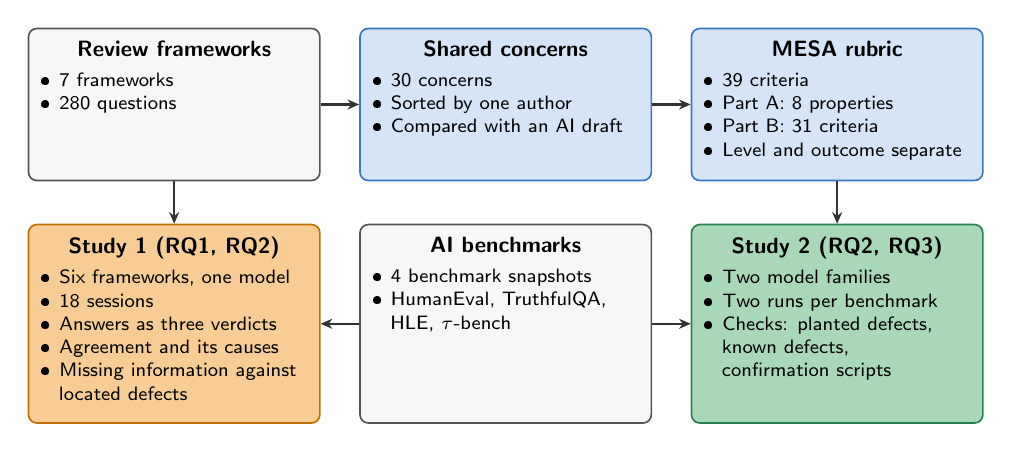
\begin{tikzpicture}
  \pgfmathsetlengthmacro{\xA}{0pt}
  \pgfmathsetlengthmacro{\xB}{\boxw+\colgap}
  \pgfmathsetlengthmacro{\xC}{2*\boxw+2*\colgap}
  \pgfmathsetlengthmacro{\yBot}{-\hTop-\rowgap}

  % top row: inputs and the mapping step
  \node[box, fill=inF, draw=inB] (F) at (\xA,0)
    {\boxcontent{\hTop}{Review frameworks}{\item 7 frameworks \item 280 questions}};
  \node[box, fill=mpF, draw=mpB] (C) at (\xB,0)
    {\boxcontent{\hTop}{Shared concerns}{\item 30 concerns \item Sorted by one author \item Compared with an AI draft}};
  \node[box, fill=mpF, draw=mpB] (R) at (\xC,0)
    {\boxcontent{\hTop}{MESA rubric}{\item 39 criteria \item Part A: 8 properties \item Part B: 31 criteria \item Level and outcome separate}};

  % bottom row: the two studies around the shared benchmarks
  \node[box, fill=sAF, draw=sAB] (S1) at (\xA,\yBot)
    {\boxcontent{\hBot}{Study 1 (RQ1, RQ2)}{\item Six frameworks, one model \item 18 sessions \item Answers as three verdicts \item Agreement and its causes \item Missing information against\newline located defects}};
  \node[box, fill=inF, draw=inB] (B) at (\xB,\yBot)
    {\boxcontent{\hBot}{AI benchmarks}{\item 4 benchmark snapshots \item HumanEval, TruthfulQA, HLE, $\tau$-bench}};
  \node[box, fill=sBF, draw=sBB] (S2) at (\xC,\yBot)
    {\boxcontent{\hBot}{Study 2 (RQ2, RQ3)}{\item Two model families \item Two runs per benchmark \item Checks: planted defects,\newline known defects,\newline confirmation scripts}};

  % arrows: straight, none cross
  \draw[link] (F.east) -- (C.west);
  \draw[link] (C.east) -- (R.west);
  \draw[link] (F.south) -- (S1.north);
  \draw[link] (R.south) -- (S2.north);
  \draw[link] (B.west) -- (S1.east);
  \draw[link] (B.east) -- (S2.west);
\end{tikzpicture}
\end{document}
